% Section content template for individual Educative lessons
% This file contains the actual content for a specific section
% Generated from Educative API section content

% Section: Use Case Diagram for the Car Rental System
% Section ID: 5990796071534592
% Section Slug: use-case-diagram-for-the-car-rental-system
% Generated: 2025-12-12T14:50:33.084103

Let's build the use case diagram for the car rental system and understand the relationship between its main actors and system functions. First , we'll define the different elements of our system, followed by the complete use case diagram and a detailed breakdown of actors and use cases.

\subsection{System}\label{Qti-BXEpmajJZjDodnlJ3}
\\
Our system is the car rental system. It manages automated vehicle reservations, returns, payments, and services for customers across multiple branches.

\subsection{Actors}\label{md76KfgJNtJS5BdYT-j00}
\\
Now, we'll define the main actors of our car rental system.

\subsubsection{Primary actor}\label{1zFV-esUXgtAy1p6d3iU0}

\begin{itemize}
\item
\protect\phantomsection\label{0pQr8bAT2qIFfVykPOF0Q}
\textbf{Customer:} The primary user, able to register, search vehicles, make and manage reservations, pick up and return vehicles, and make payments.
\end{itemize}

\subsubsection{Secondary actor}\label{Y1DsPS0gYEbLIMMIUQNR9}

\begin{itemize}
\item
\protect\phantomsection\label{VWxEHX7Tlxek5J07GC-M_}
\textbf{Receptionist:} The system operator who can perform all customer operations on behalf of a customer (e.g., register a customer, search, make/update/cancel reservations, and process payments), manage vehicle inventory, and update vehicle logs.
\end{itemize}

\subsection{Use cases}\label{uJur_2VFuND2w8FjHmU_R}
\\
This section defines the use cases for the car rental system. We have listed the use cases according to their respective interactions with a particular actor.
\begin{quote}
\textbf{Note:} Some use cases will occur multiple times because they are shared among different actors in the system.
\end{quote}
\subsubsection{Customer}\label{aiGUC0j2FdKPiNQdBQ72R}

\begin{itemize}
\item
\protect\phantomsection\label{TtidFhiccnBflOLu5JEsm}
\textbf{Register account:} To create a new customer profile with personal information in the system.
\item
\protect\phantomsection\label{Dl8lmOkrwunHC8SpMw7OI}
\textbf{Login/Logout:} To securely sign in or out of the system.
\item
\protect\phantomsection\label{L33RkQue8HdYFdcL7S26I}
\textbf{Search vehicle inventory:} To search and view available vehicles by type, model, location, or availability.
\item
\protect\phantomsection\label{dqhPs8-cPW1nPsyqOlgPo}
\textbf{Make reservation:} To reserve a vehicle for specific dates and locations, optionally selecting equipment and services.
\item
\protect\phantomsection\label{8FoieXQOjv9VNa_7Ui51s}
\textbf{Update reservation:} To request to add additional services such as ski rack, child seat, etc.
\item
\protect\phantomsection\label{h0knCgXnlF9JSVo7eZg4F}
\textbf{Cancel reservation:} To cancel an existing reservation before the scheduled pickup time.
\item
\protect\phantomsection\label{3SdQJn3ijJB6wRskgN7Zp}
\textbf{Pick up vehicle:} To complete check-in, collect a reserved vehicle from the designated branch or location.
\item
\protect\phantomsection\label{hVtXXRQnScAkTzmyX7EpI}
\textbf{Return vehicle:} To complete checkout, return a rented vehicle to an authorized branch.
\item
\protect\phantomsection\label{vCICgQYjAplZRkLTrKhy_}
\textbf{Pay bill:} To make payment for rental charges, including any extra services, fines, or late fees.
\end{itemize}

\subsubsection{Receptionist}\label{kYb2yO1H1AfeLl7xrN-o3}
\\
The following are a few use cases on behalf of customers:

\begin{itemize}
\item
\protect\phantomsection\label{TtidFhiccnBflOLu5JEsm}
\textbf{Register account:} To create a new account for customers.
\item
\protect\phantomsection\label{Dl8lmOkrwunHC8SpMw7OI}
\textbf{Login/Logout:} To securely sign in or out of the system.
\item
\protect\phantomsection\label{L33RkQue8HdYFdcL7S26I}
\textbf{Search vehicle inventory:} To search and view available vehicles by type, model, location, or availability, on behalf of a customer.
\item
\protect\phantomsection\label{dqhPs8-cPW1nPsyqOlgPo}
\textbf{Make reservation:} To reserve a vehicle for specific dates and locations, optionally selecting equipment and services on behalf of a customer.
\item
\protect\phantomsection\label{8FoieXQOjv9VNa_7Ui51s}
\textbf{Update reservation:} To add additional services such as ski rack, child seat, etc., on behalf of a customer.
\item
\protect\phantomsection\label{h0knCgXnlF9JSVo7eZg4F}
\textbf{Cancel reservation:} To cancel an existing reservation before the scheduled pickup time on behalf of a customer.
\item
\protect\phantomsection\label{DHHk-dY0cqw-p5sb-ddSs}
\textbf{Add vehicle:} To register a new vehicle in the branch inventory, specifying type and details.
\item
\protect\phantomsection\label{3lsym_AEGtHEr3mJ-yFSN}
\textbf{Remove vehicle:} To remove a vehicle from the inventory (e.g., for maintenance or decommission).
\item
\protect\phantomsection\label{Nk2Q8pizFndPt7Y6QG4AC}
\textbf{Modify vehicle info:} To update vehicle information or status (e.g., availability, service state).
\item
\protect\phantomsection\label{8FoieXQOjv9VNa_7Ui51s}
\textbf{Update reservation:} To change details of an existing reservation, such as dates, vehicle type, or selected services.
\item
\protect\phantomsection\label{4m1NEvS402Yd1OmmJzgRP}
\textbf{Update log:} To record or update significant vehicle events, such as maintenance, repairs, or status changes.
\item
\protect\phantomsection\label{by-OWITyRIZGR0md1CajX}
\textbf{Collect bill/payment:}~To accept and process customer payment upon vehicle return.
\end{itemize}

\subsubsection{Car rental system}\label{V8v_21cup7Z3JwtXhNeYX}

\begin{itemize}
\item
\protect\phantomsection\label{q50d_3X8D2ku5v1Ol8kMN}
\textbf{Send reservation notification:} To automatically send reservation confirmations to customers.
\item
\protect\phantomsection\label{6A14id-Izr5GXG7aNUBCj}
\textbf{Send reservation cancellation notification:} To notify customers when a reservation is canceled.
\item
\protect\phantomsection\label{w1ZxycMKW2uSPh8uMipiL}
\textbf{Send overdue notification:} To notify customers about overdue vehicle returns and any associated fines.
\end{itemize}

\subsection{Relationships}\label{MSkgMhl8HcMAtBoMqNim1}
\\
This section describes and justifies the system's relationships between actors and use cases. Understanding why each relationship is used will help clarify system behaviors, support extensibility, and avoid redundancy in the design.

\subsubsection{Generalization}\label{TWu5r58Co4xord30p8RBe}
\\
We'll use the generalization relationship to add, remove, or modify a vehicle. However, each vehicle type (Car, Truck, Van, Motorcycle) may have unique attributes or business rules. By using generalization:

\begin{itemize}
\item
\protect\phantomsection\label{uvMnf4mFvcXMOLRD_tC1a}
The system models ``Add vehicle'' as the common behavior.
\item
\protect\phantomsection\label{bZU0esoCZKS-tc0SEUqf5}
Each specialized use case (``Add car'', ``Add truck'', etc.) inherits from the general use case and can include additional, type-specific steps.
\item
\protect\phantomsection\label{kT4V6dcWMD8ZqtTdwzO8T}
This approach improves maintainability and scalability; only a new specialized use case must be added if a new vehicle type is introduced.
\item
\protect\phantomsection\label{SaZpGPAesSXnj30LOaJW0}
Examples:

\begin{itemize}
\item
``Add vehicle'' generalizes to ``Add car'', ``Add truck'', ``Add van'', and ``Add motorcycle''.
\item
``Remove vehicle'' generalizes to ``Remove car'', ``Remove truck'', ``Remove van'', and ``Remove motorcycle''.
\item
``Modify vehicle'' generalizes to ``Modify car'', ``Modify truck'', ``Modify van'', and ``Modify motorcycle''.
\end{itemize}
\end{itemize}

\subsubsection{Associations}\label{etla1FupQif0zTGH2yqvm}
\\
The table below shows the association relationship between actors and their use cases.

\begin{center}
{\def\LTcaptype{none} % do not increment counter
\begin{longtable}[]{@{}
>{\raggedright\arraybackslash} p{(\linewidth - 4\tabcolsep) * \real{0.3333}}
>{\raggedright\arraybackslash} p{(\linewidth - 4\tabcolsep) * \real{0.3333}}
>{\raggedright\arraybackslash} p{(\linewidth - 4\tabcolsep) * \real{0.3333}}@{}}
\toprule\noalign{}
\endhead
\bottomrule\noalign{}
\endlastfoot
\begin{minipage}[t]{\linewidth}\raggedright
\textbf{Customer}
\end{minipage} & \begin{minipage}[t]{\linewidth}\raggedright
\textbf{Receptionist}
\end{minipage} & \begin{minipage}[t]{\linewidth}\raggedright
\textbf{Car Rental System}
\end{minipage} \\
\begin{minipage}[t]{\linewidth}\raggedright
Register account
\end{minipage} & \begin{minipage}[t]{\linewidth}\raggedright
Register account
\end{minipage} & \begin{minipage}[t]{\linewidth}\raggedright
Send a reservation canceled notification
\end{minipage} \\
\begin{minipage}[t]{\linewidth}\raggedright
Login/Logout
\end{minipage} & \begin{minipage}[t]{\linewidth}\raggedright
Login/Logout
\end{minipage} & \begin{minipage}[t]{\linewidth}\raggedright
Send a reservation notification
\end{minipage} \\
\begin{minipage}[t]{\linewidth}\raggedright
Search vehicle inventory
\end{minipage} & \begin{minipage}[t]{\linewidth}\raggedright
Search vehicle inventory
\end{minipage} & \begin{minipage}[t]{\linewidth}\raggedright
Send overdue notification
\end{minipage} \\
\begin{minipage}[t]{\linewidth}\raggedright
Make reservation
\end{minipage} & \begin{minipage}[t]{\linewidth}\raggedright
Make reservation
\end{minipage} & \begin{minipage}[t]{\linewidth}\raggedright
\end{minipage} \\
\begin{minipage}[t]{\linewidth}\raggedright
Update reservation
\end{minipage} & \begin{minipage}[t]{\linewidth}\raggedright
Update reservation
\end{minipage} & \begin{minipage}[t]{\linewidth}\raggedright
\end{minipage} \\
\begin{minipage}[t]{\linewidth}\raggedright
Cancel reservation
\end{minipage} & \begin{minipage}[t]{\linewidth}\raggedright
Cancel reservation
\end{minipage} & \begin{minipage}[t]{\linewidth}\raggedright
\end{minipage} \\
\begin{minipage}[t]{\linewidth}\raggedright
Pick up vehicle
\end{minipage} & \begin{minipage}[t]{\linewidth}\raggedright
Add vehicle
\end{minipage} & \begin{minipage}[t]{\linewidth}\raggedright
\end{minipage} \\
\begin{minipage}[t]{\linewidth}\raggedright
Pay bill
\end{minipage} & \begin{minipage}[t]{\linewidth}\raggedright
Modify vehicle info
\end{minipage} & \begin{minipage}[t]{\linewidth}\raggedright
\end{minipage} \\
\begin{minipage}[t]{\linewidth}\raggedright
Return vehicle
\end{minipage} & \begin{minipage}[t]{\linewidth}\raggedright
Remove vehicle
\end{minipage} & \begin{minipage}[t]{\linewidth}\raggedright
\end{minipage} \\
\begin{minipage}[t]{\linewidth}\raggedright
\end{minipage} & \begin{minipage}[t]{\linewidth}\raggedright
Update log
\end{minipage} & \begin{minipage}[t]{\linewidth}\raggedright
\end{minipage} \\
\begin{minipage}[t]{\linewidth}\raggedright
\end{minipage} & \begin{minipage}[t]{\linewidth}\raggedright
Collect the bill/payment
\end{minipage} & \begin{minipage}[t]{\linewidth}\raggedright
\end{minipage} \\
\end{longtable}
}
\end{center}

\subsubsection{Include}\label{wr_KOJptpHbyqhuOR-04N}
\\
The ``include'' relationship is used when a use case always requires the execution of another use case as part of its flow. This avoids duplicating logic and ensures consistency.
\\
For example, whenever a customer returns a vehicle or cancels a reservation, it is always necessary to process payment for the rental, including any outstanding fees (such as late fines, damages, or extra services). By modeling ``Pay bill'' as an included use case:

\begin{itemize}
\item
\protect\phantomsection\label{ogd3IWOkuuN4SG7RL5Wz1}
The return and cancellation processes consistently enforce billing.
\item
\protect\phantomsection\label{-GgBAcM19A4z7z6lmWJE1}
Any changes to payment handling are managed in a single place (the included use case).
\end{itemize}
\\
\textbf{Examples:}

\begin{itemize}
\item
\protect\phantomsection\label{aKauXIpkDe4qYPHoZXA5y}
``Return vehicle'' includes ``Pay bill'' (the billing/payment process always occurs when returning a vehicle).
\item
\protect\phantomsection\label{5qVThbCA7l9xrTDyGbzMF}
``Make reservation'' includes ``Send reservation notification'' (a confirmation is always sent after a successful reservation).
\item
\protect\phantomsection\label{_-qINTui3oi8iKfJLQ_0X}
``Cancel reservation'' includes ``Send reservation cancellation notification'' (a notification is always sent when a reservation is canceled).
\item
\protect\phantomsection\label{xl7gRCG7gWsyIGfIySe7i}
``Return vehicle'' includes ``Send overdue notification'' (an overdue notification is sent if the vehicle is returned late).
\end{itemize}

\subsubsection{Extend}\label{gonygcR5BZIYTZCqbL6aU}
\\
An ``extend'' relationship allows optional or conditional behavior to be attached to a base use case. The extension use case is only executed if certain criteria are met.
\\
For instance, when making or updating a reservation, customers may add extras---such as rental insurance, an additional driver, Wi-Fi, or a child seat---but these are not always required. Using ``extend'':

\begin{itemize}
\item
\protect\phantomsection\label{BQTIASluUBrtKfSyyEapu}
The base reservation process remains focused and uncluttered.
\item
\protect\phantomsection\label{OSnO3y3YO-D4xph-8yq2_}
Optional features can be added or changed easily, without modifying the main flow.
\end{itemize}
\\
\textbf{Examples:}
\\
``Update reservation'' extends to the following:

\begin{itemize}
\item
\protect\phantomsection\label{e1dAZcXXJrAZiq7gihBta}
``Add rental insurance''
\item
\protect\phantomsection\label{En5QN6bscAnbyvBPxPPmo}
``Add additional driver''
\item
\protect\phantomsection\label{ccZu6k3Ph3zj2l2iYo5C8}
``Add service'' (e.g., Wi-Fi, driver, roadside assistance)
\item
\protect\phantomsection\label{hlFNsOHkrWW745i10imTR}
``Add equipment'' (e.g., child seat, ski rack, navigation system)
\end{itemize}
\\
These extensions are invoked only if the customer requests them during the reservation or update process.

\subsection{Use case diagram}\label{UgT_2EAECB-8vZnusb4uT}
\\
Here's the use case diagram for the car rental system:

\begin{figure}[htbp]
 \centering
 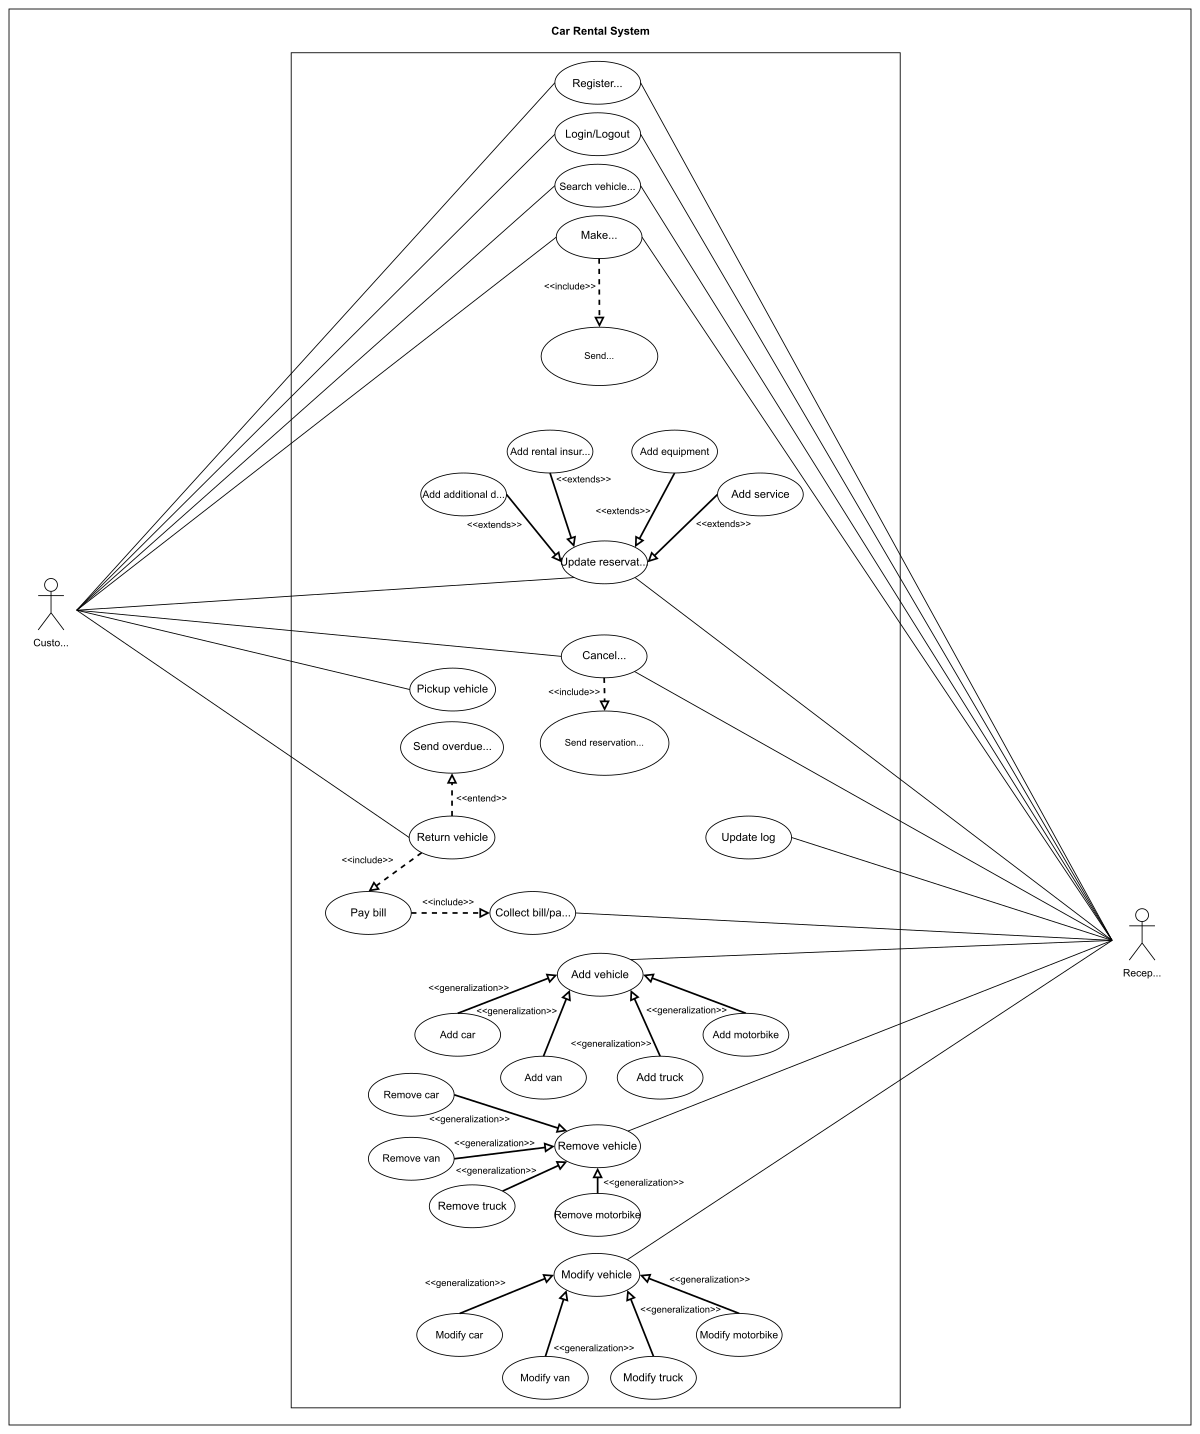
\includegraphics[width=0.5\textwidth]{Images/chapter_15/section_5990796071534592/6164280565956608.png}
 \caption{The use case diagram of the car rental system}
\end{figure}

In the next lesson, we'll discuss the class diagram with a detailed explanation of all classes and their relationship with each other.

% End of section content